\part{Annexe}

\chapter{Photos illustratives d'équipements informatique}

\begin{figure}[H]
	\centering
	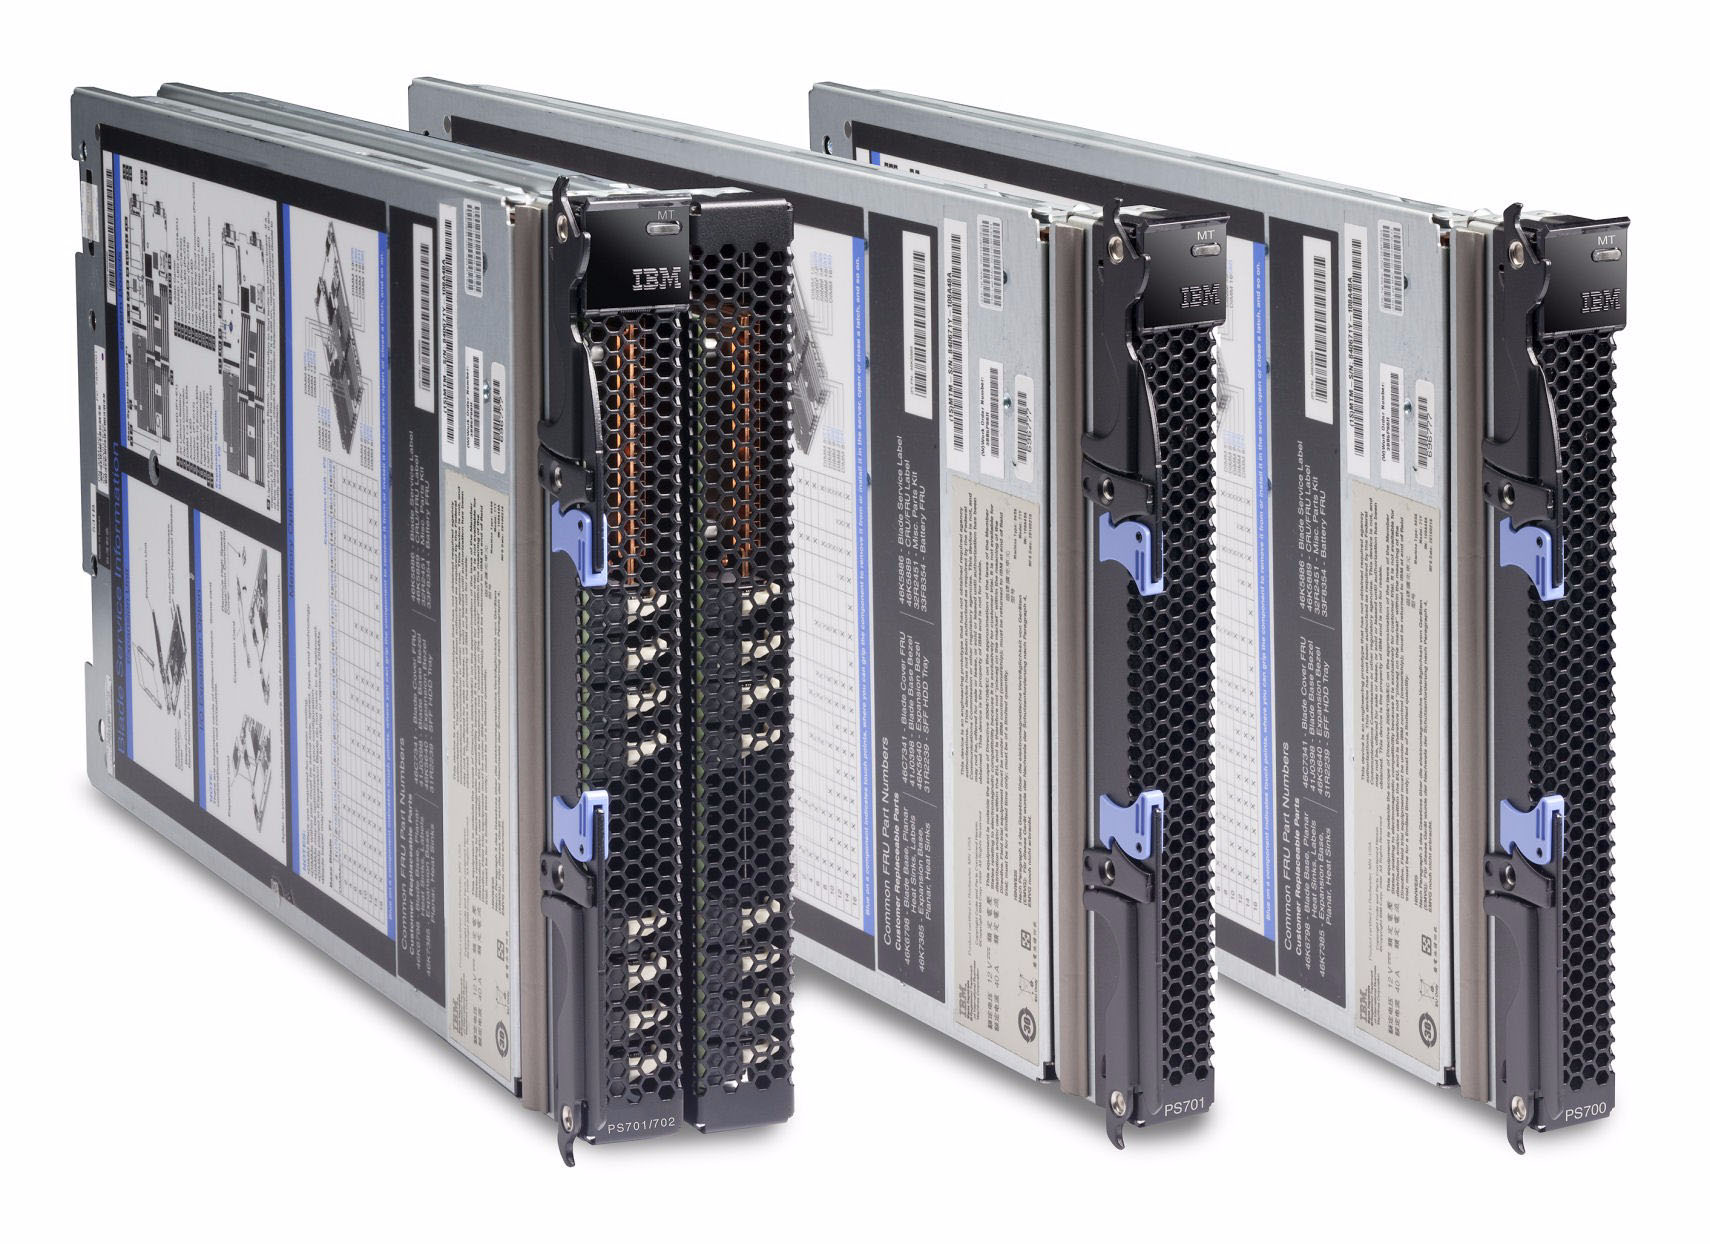
\includegraphics[width=0.6\textwidth]{resource/img/blade}
	\caption{Trois serveurs lames (\emph{blade server} en anglais)}
\end{figure}

\begin{figure}[H]
	\centering
	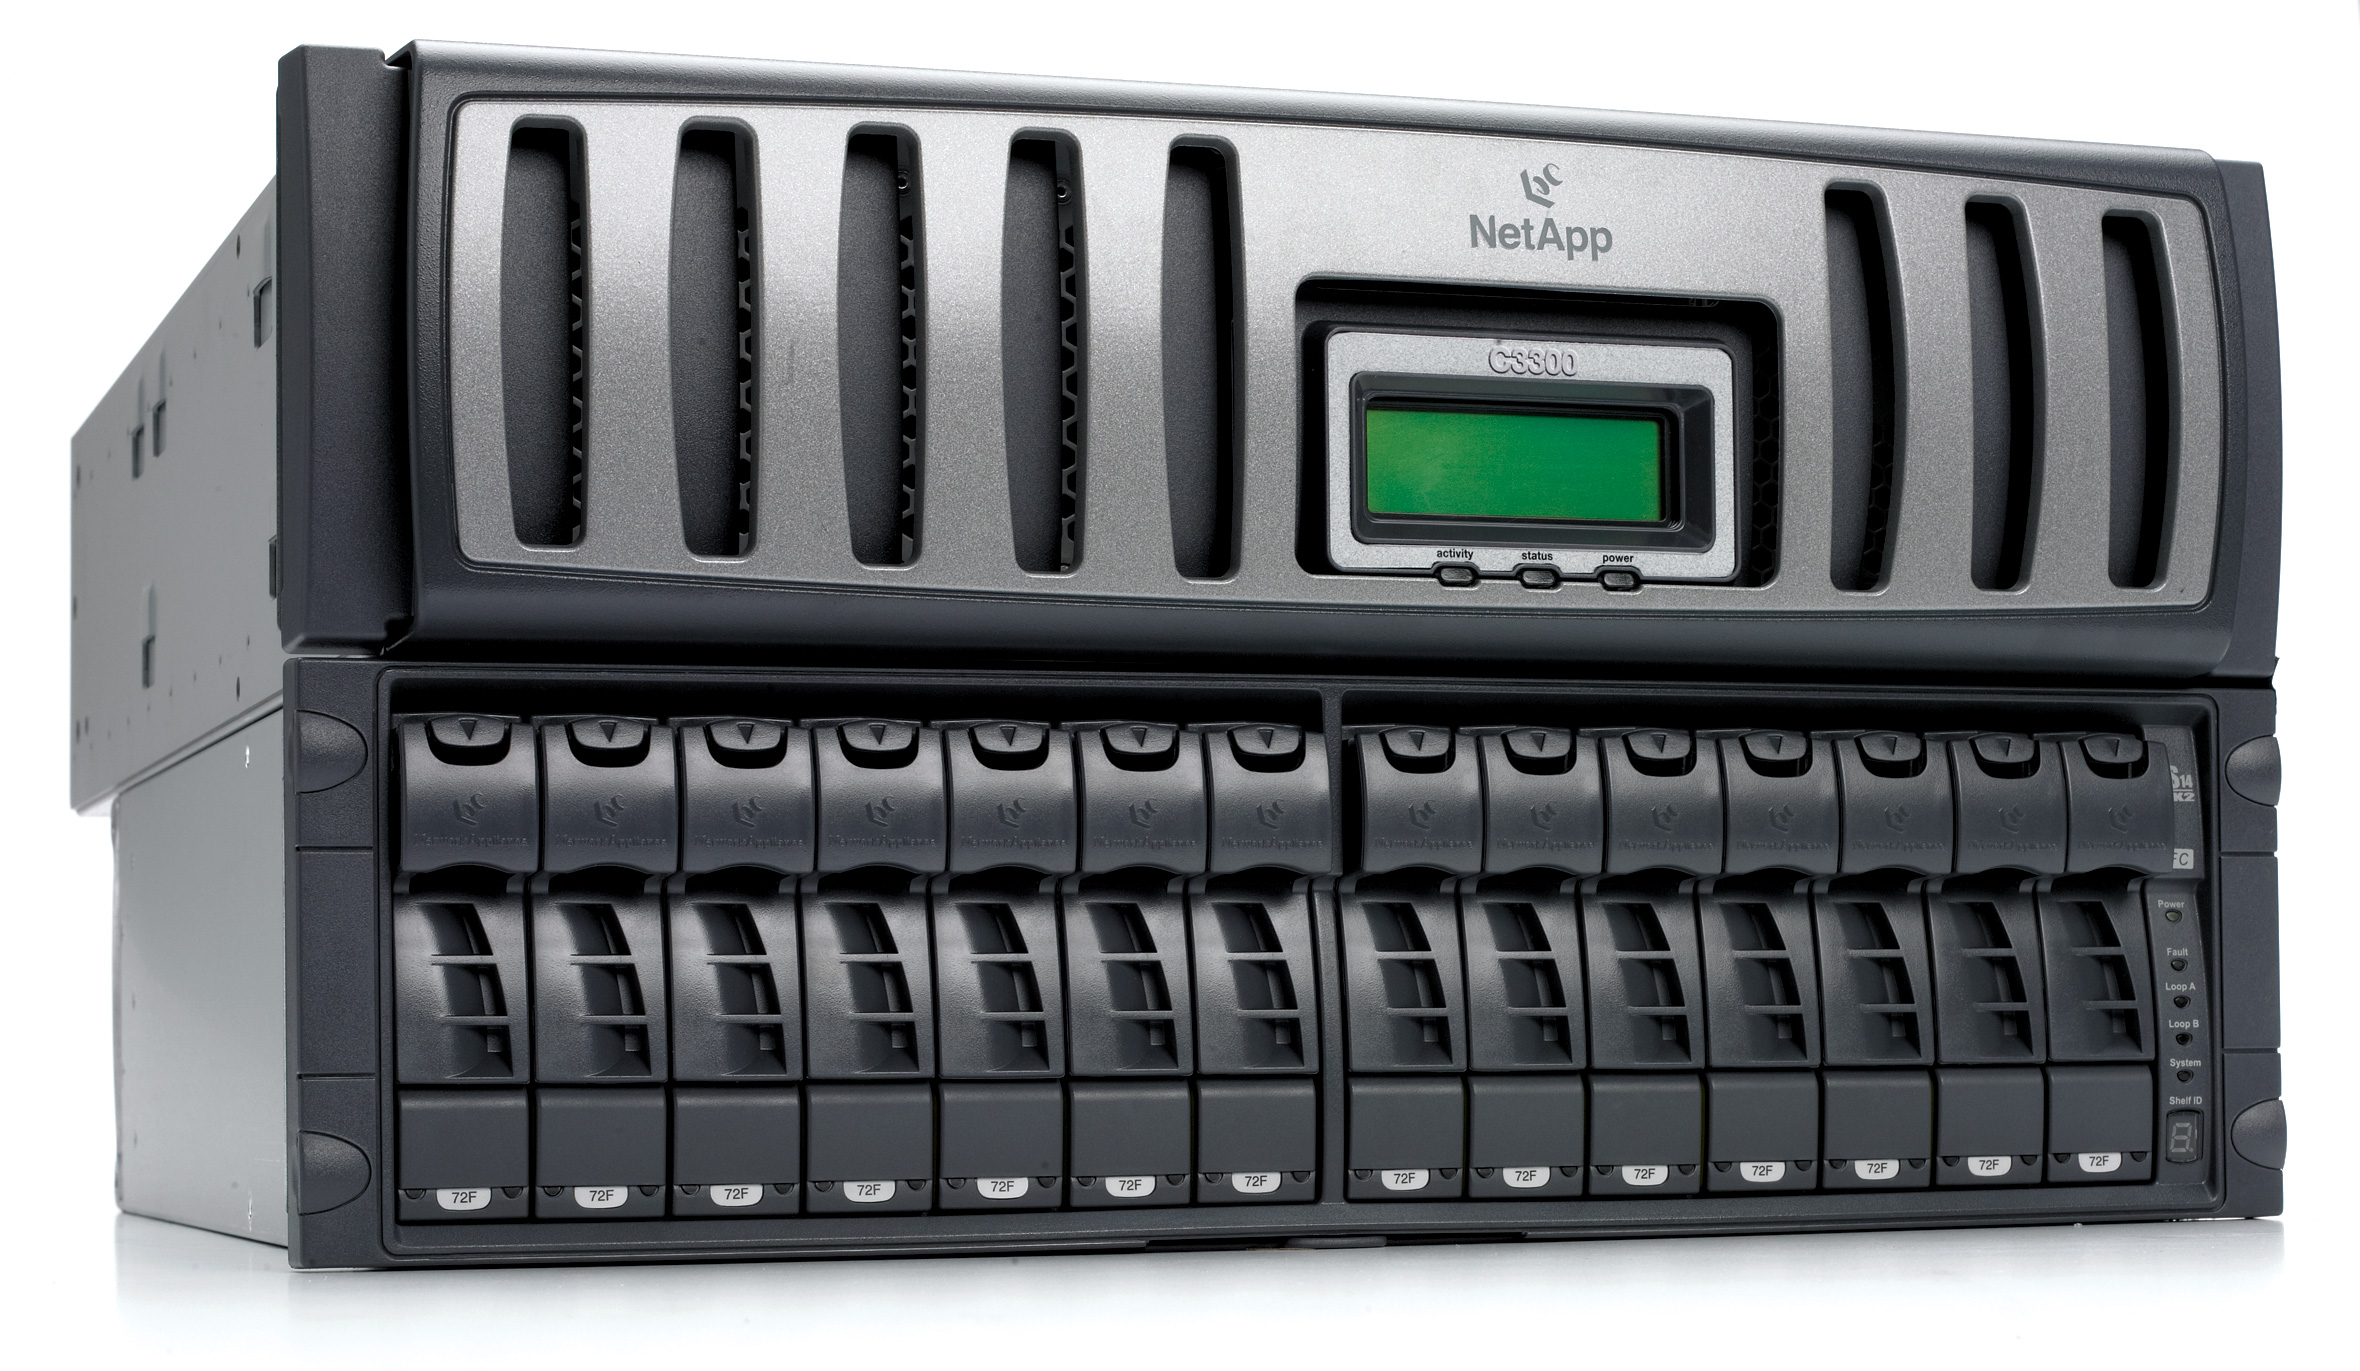
\includegraphics[width=0.6\textwidth]{resource/img/netapp_c3300}
	\caption{Baie de disque NetApp C3300 contenant 14 disques durs}
	\label{netapp}
\end{figure}

\begin{figure}[H]
	\centering
	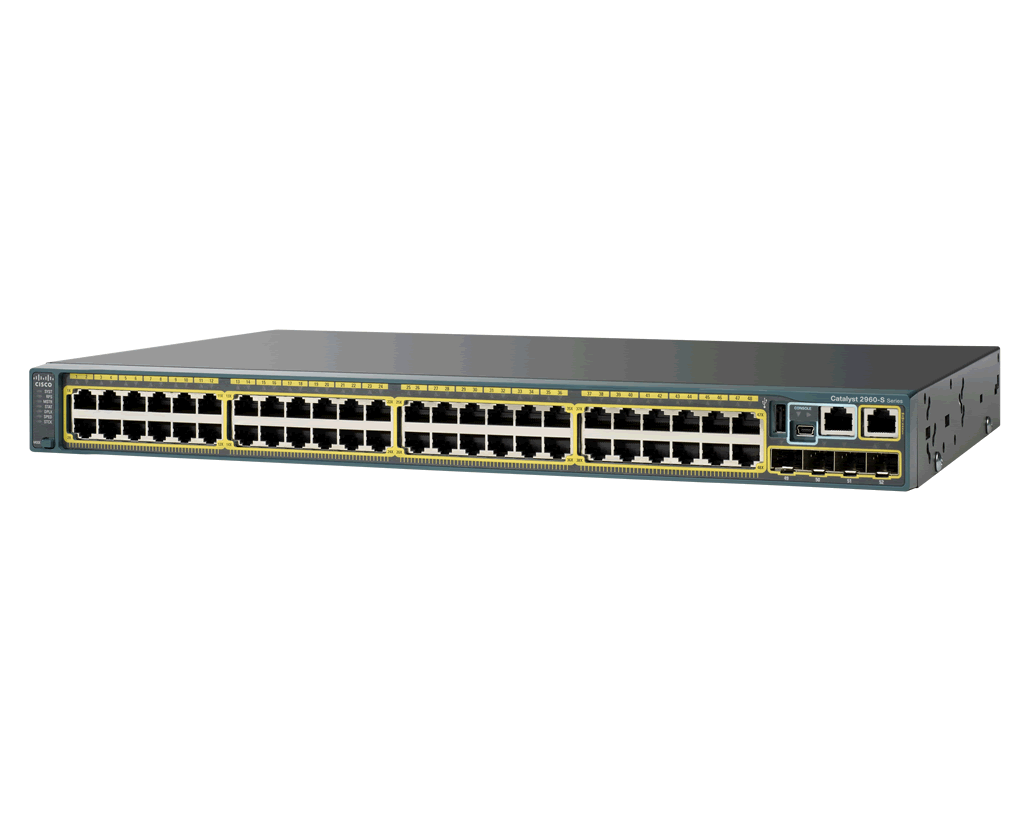
\includegraphics[width=0.6\textwidth]{resource/img/cisco-switch}
	\caption{Switch Cisco WS-C2960}
\end{figure}

\begin{figure}[H]
	\centering
	\includegraphics[width=0.6\textwidth]{resource/img/DC}
	\caption{Plusieurs baies de serveur (\emph{rack} en anglais) dans un Data Center}
	\label{datacenter}
\end{figure}


\chapter{Benchmark des I/Os disque sous Xen}

\paragraph*{}
Ces benchmarks ont été réalisés dans le but l'impact des différentes versions du noyau linux
(en DomU) sur les performances d'I/O disque des VM Xen.


\section{Noyau linux 2.6.32-xen}

\subsection*{En lecture}

\begin{figure}[H]
	\centering
	\includegraphics[angle=-90,width=0.8\textwidth]{resource/plot/iozone-2_6_32-debian-xen-withoutcache-withoutbarrier_out_reads}
	\caption{Cache d'écriture: \textbf{désactivé}   -   Barrière d'écriture: \textbf{désactivée}}
\end{figure}

\begin{figure}[H]
	\centering
	\includegraphics[angle=-90,width=0.8\textwidth]{resource/plot/iozone-2_6_32-debian-xen-withcache-withoutbarrier_out_reads}
	\caption{Cache d'écriture: \textbf{activé}   -   Barrière d'écriture: \textbf{désactivée}}
\end{figure}

\begin{figure}[H]
	\centering
	\includegraphics[angle=-90,width=0.8\textwidth]{resource/plot/iozone-2_6_32-debian-xen-withcache-withbarrier_out_reads}
	\caption{Cache d'écriture: \textbf{activé}   -   Barrière d'écriture: \textbf{activée}}
\end{figure}

\subsection*{En écriture}

\begin{figure}[H]
	\centering
	\includegraphics[angle=-90,width=0.8\textwidth]{resource/plot/iozone-2_6_32-debian-xen-withoutcache-withoutbarrier_out_writes}
	\caption{Cache d'écriture: \textbf{désactivé}   -   Barrière d'écriture: \textbf{désactivée}}
\end{figure}

\begin{figure}[H]
	\centering
	\includegraphics[angle=-90,width=0.8\textwidth]{resource/plot/iozone-2_6_32-debian-xen-withcache-withoutbarrier_out_writes}
	\caption{Cache d'écriture: \textbf{activé}   -   Barrière d'écriture: \textbf{désactivée}}
\end{figure}

\begin{figure}[H]
	\centering
	\includegraphics[angle=-90,width=0.8\textwidth]{resource/plot/iozone-2_6_32-debian-xen-withcache-withbarrier_out_writes}
	\caption{Cache d'écriture: \textbf{activé}   -   Barrière d'écriture: \textbf{activée}}
\end{figure}

\section{Noyau linux 3.1}

\subsection*{En lecture}

\begin{figure}[H]
	\centering
	\includegraphics[angle=-90,width=0.8\textwidth]{resource/plot/iozone-3_1-linus-withoutcache-withoutbarrier_out_reads}
	\caption{Cache d'écriture: \textbf{désactivé}   -   Barrière d'écriture: \textbf{désactivée}}
\end{figure}

\begin{figure}[H]
	\centering
	\includegraphics[angle=-90,width=0.8\textwidth]{resource/plot/iozone-3_1-linus-withcache-withoutbarrier_out_reads}
	\caption{Cache d'écriture: \textbf{activé}   -   Barrière d'écriture: \textbf{désactivée}}
\end{figure}

\begin{figure}[H]
	\centering
	\includegraphics[angle=-90,width=0.8\textwidth]{resource/plot/iozone-3_1-linus-withcache-withbarrier_out_reads}
	\caption{Cache d'écriture: \textbf{activé}   -   Barrière d'écriture: \textbf{activée}}
\end{figure}

\subsection*{En écriture}

\begin{figure}[H]
	\centering
	\includegraphics[angle=-90,width=0.8\textwidth]{resource/plot/iozone-3_1-linus-withoutcache-withoutbarrier_out_writes}
	\caption{Cache d'écriture: \textbf{désactivé}   -   Barrière d'écriture: \textbf{désactivée}}
\end{figure}

\begin{figure}[H]
	\centering
	\includegraphics[angle=-90,width=0.8\textwidth]{resource/plot/iozone-3_1-linus-withcache-withoutbarrier_out_writes}
	\caption{Cache d'écriture: \textbf{activé}   -   Barrière d'écriture: \textbf{désactivée}}
\end{figure}

\begin{figure}[H]
	\centering
	\includegraphics[angle=-90,width=0.8\textwidth]{resource/plot/iozone-3_1-linus-withcache-withbarrier_out_writes}
	\caption{Cache d'écriture: \textbf{activé}   -   Barrière d'écriture: \textbf{activée}}
\end{figure}

\section{Noyau linux 3.2}

\subsection*{En lecture}

\begin{figure}[H]
	\centering
	\includegraphics[angle=-90,width=0.8\textwidth]{resource/plot/iozone-3_2-linus-withoutcache-withoutbarrier_out_reads}
	\caption{Cache d'écriture: \textbf{désactivé}   -   Barrière d'écriture: \textbf{désactivée}}
\end{figure}

\begin{figure}[H]
	\centering
	\includegraphics[angle=-90,width=0.8\textwidth]{resource/plot/iozone-3_2-linus-withcache-withoutbarrier_out_reads}
	\caption{Cache d'écriture: \textbf{activé}   -   Barrière d'écriture: \textbf{désactivée}}
\end{figure}

\begin{figure}[H]
	\centering
	\includegraphics[angle=-90,width=0.8\textwidth]{resource/plot/iozone-3_2-linus-withcache-withbarrier_out_writes}
	\caption{Cache d'écriture: \textbf{activé}   -   Barrière d'écriture: \textbf{activée}}
\end{figure}

\subsection*{En écriture}

\begin{figure}[H]
	\centering
	\includegraphics[angle=-90,width=0.8\textwidth]{resource/plot/iozone-3_2-linus-withoutcache-withoutbarrier_out_writes}
	\caption{Cache d'écriture: \textbf{désactivé}   -   Barrière d'écriture: \textbf{désactivée}}
\end{figure}

\begin{figure}[H]
	\centering
	\includegraphics[angle=-90,width=0.8\textwidth]{resource/plot/iozone-3_2-linus-withcache-withoutbarrier_out_writes}
	\caption{Cache d'écriture: \textbf{activé}   -   Barrière d'écriture: \textbf{désactivée}}
\end{figure}

\begin{figure}[H]
	\centering
	\includegraphics[angle=-90,width=0.8\textwidth]{resource/plot/iozone-3_2-linus-withcache-withbarrier_out_writes}
	\caption{Cache d'écriture: \textbf{activé}   -   Barrière d'écriture: \textbf{activée}}
\end{figure}
